\documentclass[10pt,a4paper, margin=1in]{article}
\usepackage{fullpage}
\usepackage{amsfonts, amsmath, pifont}
\usepackage{amsthm}
\usepackage{graphicx}
\usepackage{float}

\usepackage{tkz-euclide}
\usepackage{tikz}
\usepackage{pgfplots}
\pgfplotsset{compat=1.13}
\usepackage{listings}

\usepackage{geometry}
 \geometry{
 a4paper,
 total={210mm,297mm},
 left=10mm,
 right=10mm,
 top=10mm,
 bottom=16mm,
 }
 % Write both of your names here. Fill exxxxxxx with your ceng mail address.
 \author{
  Akçan, Batuhan\\
  \texttt{e2580181@ceng.metu.edu.tr}
  \and
  Sönmezer, Mert\\
  \texttt{e2516920@ceng.metu.edu.tr}
}

\title{CENG 384 - Signals and Systems for Computer Engineers \\
Spring 2024 \\
Homework 1}
\begin{document}
\maketitle



\noindent\rule{19cm}{1.2pt}

\begin{enumerate}

\item %write the solution of q1
    \begin{enumerate}
    % Write your solutions in the following items.
    \item %write the solution of q1a
    Multiply numerator and denominator by $2-2\sqrt{3}j.$\vspace{0.3cm}\\
    $z = \frac{\sqrt{2}+\sqrt{2}j}{2+2\sqrt{3}j} = \frac{2\sqrt{2}-2\sqrt{6} + (2\sqrt{2}-2\sqrt{6})j}{4-12j^2} = \frac{(2\sqrt{2}-2\sqrt{6})(1+j)}{16} = \frac{\sqrt{2}-\sqrt{6}}{8} + \frac{\sqrt{2}-\sqrt{6}}{8}j.$\vspace{0.3cm}\\
    $Re\{z\} = \frac{\sqrt{2}-\sqrt{6}}{8} \approx -0.13.$\vspace{0.3cm}\\
    $Im\{z\} = \frac{\sqrt{2}-\sqrt{6}}{8} \approx -0.13.$\vspace{0.3cm}
    \item %write the solution of q1b
    We can express $z$ as $z = a + bj$, where\vspace{0.3cm}\\
    $a = \frac{\sqrt{2}-\sqrt{6}}{8} \;,\; b = \frac{\sqrt{2}-\sqrt{6}}{8}.$\vspace{0.3cm}\\
    The magnitude is:\vspace{0.3cm}\\
    $r = \sqrt{a^2+b^2} = \sqrt{2a^2} = |a|\sqrt{2} = |\frac{\sqrt{2}-\sqrt{6}}{8}| \cdot \sqrt{2} = |\frac{2-2\sqrt{3}}{8}| = |\frac{1-\sqrt{3}}{4}| \approx 0.18.$\vspace{0.3cm}\\
    The phase is:\vspace{0.3cm}\\
    $\theta = arctan(\frac{b}{a}) = arctan1 = \frac{\pi}{4}.$\vspace{0.3cm}\\
    \end{enumerate}

\item %write the solution of q2
$t=0 \rightarrow y(0) = x(-2).$\vspace{0.3cm}\\
$t=2 \rightarrow y(2) = x(-1).$\vspace{0.3cm}\\
$t=4 \rightarrow y(4) = x(0).$\vspace{0.3cm}\\
$t=6 \rightarrow y(6) = x(1).$\vspace{0.3cm}\\
$t=8 \rightarrow y(8) = x(2).$\vspace{0.3cm}\\

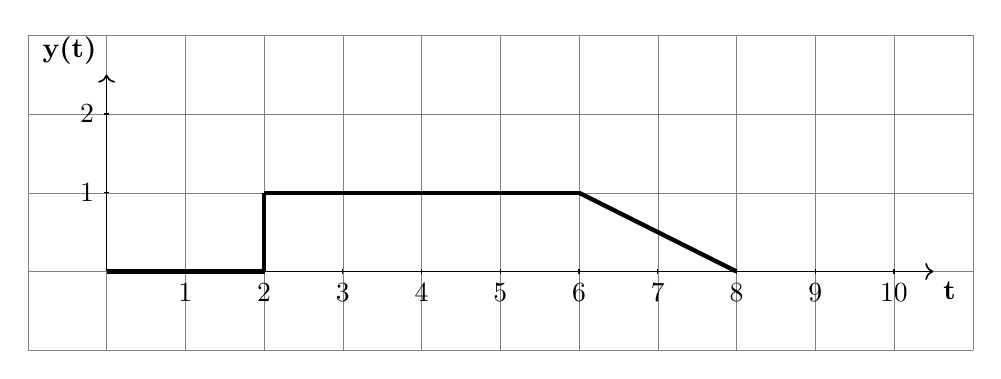
\begin{tikzpicture}
\draw[step=1cm,gray,ultra thin] (-1,-1) grid (11,3);

\draw[semithick,->] (0,0) -- (10.5,0) node[anchor=north west] {\textbf{t}};
\draw[semithick,->] (0,0) -- (0,2.5) node[anchor=south east] {\textbf{y(t)}};

\foreach \x in {1,2,3,4,5,6,7,8,9,10}
   \draw (\x cm,1pt) -- (\x cm,-1pt) node[anchor=north] {$\x$};
\foreach \y in {1,2}
    \draw (1pt,\y cm) -- (-1pt,\y cm) node[anchor=east] {$\y$};
    
\draw[ultra thick] (0,0) -- (2,0);
\draw[ultra thick] (2,0) -- (2,1);
\draw[ultra thick] (2,1) -- (6,1);
\draw[ultra thick] (6,1) -- (8,0);
\end{tikzpicture}\vspace{0.3cm}\\

\item %write the solution of q3
    \begin{enumerate}
    % Write your solutions in the following items.
    \item %write the solution of q3a
    $x[n] = \delta[n+3] - \delta[n+2] - \delta[n+1] - \delta[n] + \delta[n-1] + 2\delta[n-2] + \delta[n-3].$\vspace{0.3cm}
    \item %write the solution of q3b
    For $n<=-5,\; y[n]=0.$ \vspace{0.3cm}\\
    $n=-4 \rightarrow y[-4] = x[-6]+x[5]=0.$\vspace{0.3cm}\\
    $n=-3 \rightarrow y[-3] = x[-4]+x[4]=0.$\vspace{0.3cm}\\
    $n=-2 \rightarrow y[-2] = x[-2]+x[3]=0.$\vspace{0.3cm}\\
    $n=-1 \rightarrow y[-1] = x[0]+x[2]=1.$\vspace{0.3cm}\\
    $n=0 \rightarrow y[0] = x[2]+x[1]=3.$\vspace{0.3cm}\\
    $n=1 \rightarrow y[1] = x[4]+x[0]=-1.$\vspace{0.3cm}\\
    $n=2 \rightarrow y[2] = x[6]+x[-1]=-1.$\vspace{0.3cm}\\
    $n=3 \rightarrow y[3] = x[8]+x[-2]=-1.$\vspace{0.3cm}\\
    $n=4 \rightarrow y[4] = x[10]+x[-3]=1.$\vspace{0.3cm}\\
    For $n>=5,\; y[n]=0.$\vspace{0.3cm}\\
    
    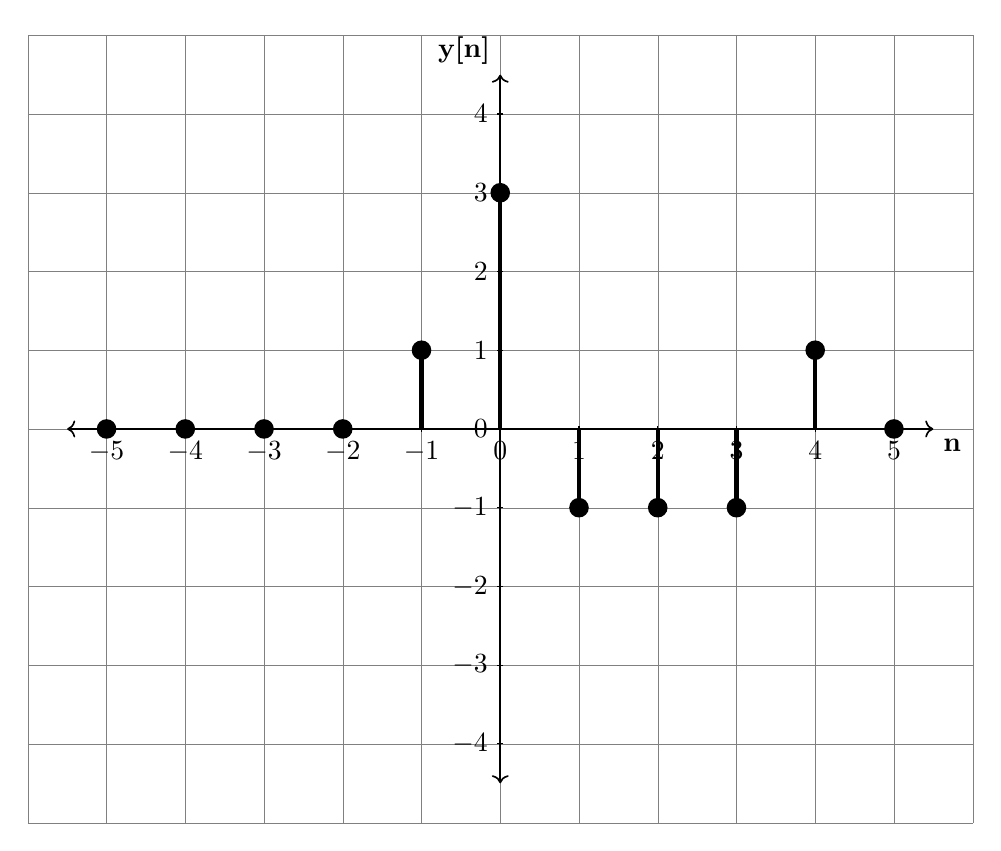
\begin{tikzpicture}
\draw[step=1cm,gray,ultra thin] (-6,-5) grid (6,5);

\draw[semithick,->] (0,0) -- (5.5,0) node[anchor=north west] {\textbf{n}};
\draw[semithick,->] (0,0) -- (0,4.5) node[anchor=south east] {\textbf{y[n]}};
\draw[semithick,->] (0,0) -- (-5.5,0);
\draw[semithick,->] (0,0) -- (0,-4.5);

\foreach \x in {-5,-4,-3,-2,-1,0,1,2,3,4,5}
   \draw (\x cm,1pt) -- (\x cm,-1pt) node[anchor=north] {$\x$};
\foreach \y in {-4,-3,-2,-1,0,1,2,3,4}
    \draw (1pt,\y cm) -- (-1pt,\y cm) node[anchor=east] {$\y$};
    
\draw[ultra thick] (-1,0) -- (-1,1);
\draw[ultra thick] (0,0) -- (0,3);
\draw[ultra thick] (1,0) -- (1,-1);
\draw[ultra thick] (2,0) -- (2,-1);
\draw[ultra thick] (3,0) -- (3,-1);
\draw[ultra thick] (4,0) -- (4,1);

\node at (-5,0)[circle,fill,inner sep=2.5pt]{};
\node at (-4,0)[circle,fill,inner sep=2.5pt]{};
\node at (-3,0)[circle,fill,inner sep=2.5pt]{};
\node at (-2,0)[circle,fill,inner sep=2.5pt]{};
\node at (-1,1)[circle,fill,inner sep=2.5pt]{};
\node at (0,3)[circle,fill,inner sep=2.5pt]{};
\node at (1,-1)[circle,fill,inner sep=2.5pt]{};
\node at (2,-1)[circle,fill,inner sep=2.5pt]{};
\node at (3,-1)[circle,fill,inner sep=2.5pt]{};
\node at (4,1)[circle,fill,inner sep=2.5pt]{};
\node at (5,0)[circle,fill,inner sep=2.5pt]{};
\end{tikzpicture}\vspace{0.3cm}\\
    
	\item %write the solution of q3c
	$y[n] = \delta[n+1] + 3\delta[n] - \delta[n-1] - \delta[n-2] - \delta[n-3] + \delta[n-4].$\vspace{0.3cm}\\
    \end{enumerate}

\item %write the solution of q4
    \begin{enumerate}   
    % Write your solutions in the following items.
    \item %write the solution of q4a
    If $x_1[n]$ is periodic, then \\
    $$x_1[n]=x_1[n+N]\rightarrow\cos{(\frac{5\pi n}{2})}=\cos{(\frac{5\pi n}{2}+\frac{5\pi N}{2})}$$ \\
    The equation above implies the following equation: \\ 
    $$\frac{5\pi n}{2}+2\pi k_1 = \frac{5\pi n}{2}+\frac{5\pi N}{2}+2\pi k_2$$ where $k_1,k_2\in Z$\\
    $$\frac{5\pi N}{2}=2\pi (k_2-k_1)$$
    Define $k_2-k_1=k_3$. Then, \\
    $$\frac{N}{k_3}=\frac{4}{5}$$
    where $k_3 \in Z$. Since we obtained two integers $N$ and $k_3$, the function is periodic, and its fundamental period is $N=4$ for $k_3=5$.\\
    \item %write the solution of q4b
    If $x_2[n]$ is periodic, then \\
    $$x_2[n]=x_2[n+N]\rightarrow\sin{(5n)}=\sin{(5n+5N)}$$
    The equation above implies the following equation: \\ 
    $$5n+2\pi k_1=5n+5N+2\pi k_2$$ where $k_1,k_2\in Z$.\\
    $$5N=2\pi (k_2-k_1)$$
    Define $k_2-k_1=k_3$. Then, \\
    $$\frac{N}{k_3}=\frac{2\pi}{5}$$ where $k_3\in Z$. We cannot find any integer values for both $N$ and $k_3$ satisfying the equation above. Thus, the function is not periodic. \\
    \item %write the solution of q4c
    If $x_3(t)$ is periodic, then
    $$x_3(t)=x_3(t+T)\rightarrow 5\sin{(4t+\frac{\pi}{3})}=5\sin{(4(t+T)+\frac{\pi}{3})}$$
    The above equation directly implies that
    $$4t+\frac{\pi}{3}+2k_1\pi=4t+4T+\frac{\pi}{3}+2k_2\pi$$ where $k_1,k_2\in Z$.\\
    $$4T=2\pi (k_1-k_2)$$
    Define $k_3=k_1-k_2$. Hence,
    $$T=\frac{\pi k_3}{2}$$ where $k_3\in Z$.The function is periodic, and its fundamental period is $T=\frac{\pi}{2}$ for $k_3=1$. \\
    \end{enumerate}

\item %write the solution of q5   
    First, notice that $\delta (\alpha t)$ is an even function since it is symmetric with respect to the $y$ axis. This directly implies that
    $$\delta (t)=\delta (-t)$$
    That is, the sign of $\alpha$ doesn't matter in the given expression. Then, we know the following equation
    $$\int_{-\infty}^{\infty}x(\tau)\delta (\tau)d\tau=x(0)$$
    Using a similar logic, let's prove the given expression.
    $$\int_{-\infty}^{\infty}x(\tau)\delta (a\tau)d\tau=\int_{-\infty}^{\infty}x(\frac{\tau^{\prime}}{a})\delta (\tau^{\prime})\frac{1}{a}d\tau^{\prime}$$
    if $\tau$ is replaced with $\frac{\tau^\prime}{a}$ by the rule of integration by substitution. Then,
    $$\int_{-\infty}^{\infty}x(\frac{\tau^{\prime}}{a})\delta (\tau^{\prime})\frac{1}{a}d\tau^{\prime}=\frac{1}{a}\int_{-\infty}^{\infty}x(\frac{\tau^{\prime}}{a})\delta (\tau^{\prime})d\tau^{\prime}=\frac{1}{a}x(\frac{0}{a})=\frac{1}{a}x(0)$$
    Notice that
    $$\frac{1}{a}x(0)=\frac{1}{a}\int_{-\infty}^{\infty}x(\tau)\delta (\tau)d\tau$$
    Therefore, since $\delta (a t)$ and $\frac{1}{|a|}\delta (t)$ have the same effect on any function $x(t)$, $\delta (a t)=\frac{1}{|a|}\delta (t)$ for $a\neq 0$.\\
\item %write the solution of q6
    \begin{enumerate}
    % Write your solutions in the following items.
    \item %write the solution of q6a
    To find the difference equation for $S$, let's first find $y_1[n-2]$
    $$y_1[n-2]=4x_1[n-2]+2x_1[n-3]$$
    Then, we need to calculate $y_2[n]$ in terms of $x_1[n]$.
    $$y_2[n]=4x_1[n-2]+2x_1[n-3]$$
    This gives us the difference equation for the overall system $S$ as the following:
    $$S:y[n]=4x[n-2]+2x[n-3]$$\\
    \item %write the solution of q6b
    If the order of the series connection of $S1$ and $S2$ were reversed, then
    $$S2:y_1[n]=x_1[n-2]$$
    $$S1:y_2[n]=4x_1[n-2]+2x_1[n-3]$$
    Therefore, the overall system $S$ would be
    $$S:y[n]=4x[n-2]+2x[n-3]$$
    That equation is the same as the one found in part $a$. Therefore, it can be concluded that the series connection of the subsystems $S1$ and $S2$ is commutative. \\
    \item %write the solution of q6c
    A system is called linear if and only if it satisfies the superposition property. Let's check the superposition property on the system given.
    $$y_1[n]=4x_1[n-2]+2x_1[n-3]$$
    $$y_2[n]=4x_2[n-2]+2x_2[n-3]$$
    $$\alpha y_1[n]+\beta y_2[n]=4\alpha x_1[n-2]+2\alpha x_1[n-3]+4\beta x_2[n-2]+2\beta x_2[n-3]$$
    The superposition of the two inputs is as the following:
    $$x=\alpha x_1+\beta x_2$$
    Now, let's give the superposition of the inputs found above to the system as the input, and check whether it is linear or not.
    $$4(\alpha x_1[n-2]+\beta x_2[n-2])+2(\alpha x_1[n-2]+\beta x_2[n-2])=4\alpha x_1[n-2]+2\alpha x_1[n-3]+4\beta x_2[n-2]+2\beta x_2[n-3]$$
    Since the expression found above is equal to the expression $\alpha y_1[n]+\beta y_2[n]$, the system is linear. \\
    \item %write the solution of q6d
    To check whether the system is time invariant, let's shift the input of the system by the time amount
    of $n_0$ to define a new input $x[n]:=x[n-n_0]$. Then, the corresponding output becomes
    $$4x[n-n_0-2]+2x[n-n_0-3]$$
    Notice that the output above is equal to the expression, which is $y[n-n_0]=4x[n-n_0-2]+2x[n-n_0-3]$. Consequently, the provided system is time invariant.
    \end{enumerate}
    
\item %write the solution of q7
    \begin{enumerate}
    % Write your solutions in the following items.
    \item %write the solution of q7a
\begin{lstlisting}
import sympy as sp
    
n = sp.Symbol("n")
alpha = sp.Symbol("alpha")
beta = sp.Symbol("beta")

x1 = sp.Function("x1", real=False)(n)
x2 = sp.Function("x2", real=False)(n)
x3 = alpha * x1 + beta * x2

y1 = x1 * n
y2 = x2 * n
y3_1 = x3 * n
y3_2 = alpha * y1 + beta * y2


if y3_1.equals(y3_2):
    print("The given system is a Linear system")
else:
    print("The given system is a Non-Linear system")
\end{lstlisting}\vspace{0.3cm}
    
    \item %write the solution of q7b
\begin{lstlisting}
import sympy as sp

n = sp.Symbol("n")
alpha = sp.Symbol("alpha")
beta = sp.Symbol("beta")

x1 = sp.Function("x1", real=False)(n)
x2 = sp.Function("x2", real=False)(n)
x3 = alpha * x1 + beta * x2

y1 = x1 ** 2
y2 = x2 ** 2
y3_1 = x3 ** 2
y3_2 = alpha * y1 + beta * y2

if y3_1.equals(y3_2):
    print("The given system is a Linear system")
else:
    print("The given system is a Non-Linear system")
\end{lstlisting}  
    \end{enumerate}  

\end{enumerate}


\end{document}
